\documentclass[10pt, a4paper]{article}
% The next line loads some packages you will need

\usepackage{graphicx, amsmath, amssymb, fancyhdr, setspace,titlesec,enumitem,indentfirst,hyperref}
\usepackage[labelfont=bf]{caption}
\usepackage[table]{xcolor}
\hypersetup{
    colorlinks=true,
    linkcolor=blue,
    filecolor=blue,      
    urlcolor=blue,
    pdftitle={Overleaf Example},
    pdfpagemode=FullScreen,
    }

% Page formatting
\addtolength{\textwidth}{5mm}
\addtolength{\textheight}{12mm}
\addtolength{\topmargin}{-10mm}
\pretolerance = 10000000
\setlength{\parindent}{23pt}
% \setlength{\parskip}{\baselineskip}
\onehalfspacing   

% Header / footer
\pagestyle{fancy}
\lhead{Himanshu Madan, 201501359}
\chead{}
\rhead{\em MATH 5747M, assignment 2}
\lfoot{}
\cfoot{\thepage}
\rfoot{}
\setlength{\headheight}{20pt}
\renewcommand{\headrulewidth}{0.4pt}
\renewcommand{\footrulewidth}{0pt}

% \titlespacing\section{0pt}{10pt plus 4pt minus 2pt}{0pt plus 0pt minus 0pt}

\begin{document}
\begin{center}
\textbf{\Large Decision Science Using MCDA} \\
Based on module LUBS 5308M Business Analytics and Decision Science \\
Lectured by Dr. Richard Hodgett \\
\end{center}

\section*{Introduction}
The objective of this report is to explain two different but prominent \textbf{Multi Criteria Decision Analysis} techniques:
\begin{itemize}[noitemsep]
    \item \textbf{Analytical Hierarchy Process }(AHP)
    \item \textbf{Technique for Order Preference by Similarity to Ideal Solutions }(TOPSIS)
\end{itemize}
MCDA techniques allow us to choose the most suitable alternative amongst all the options available using the information available.\\
In MCDA, we have :
\begin{enumerate}[noitemsep]
    \item A goal to be achieved. Ex: choose a car to buy.
    \item Multiple alternatives available. Ex: Ford Fiesta, Audi A8, BMW 530d.
    \item Several criteria influencing our decision making. Ex: cost, engine power etc.
\end{enumerate}
\begin{figure}[h]
	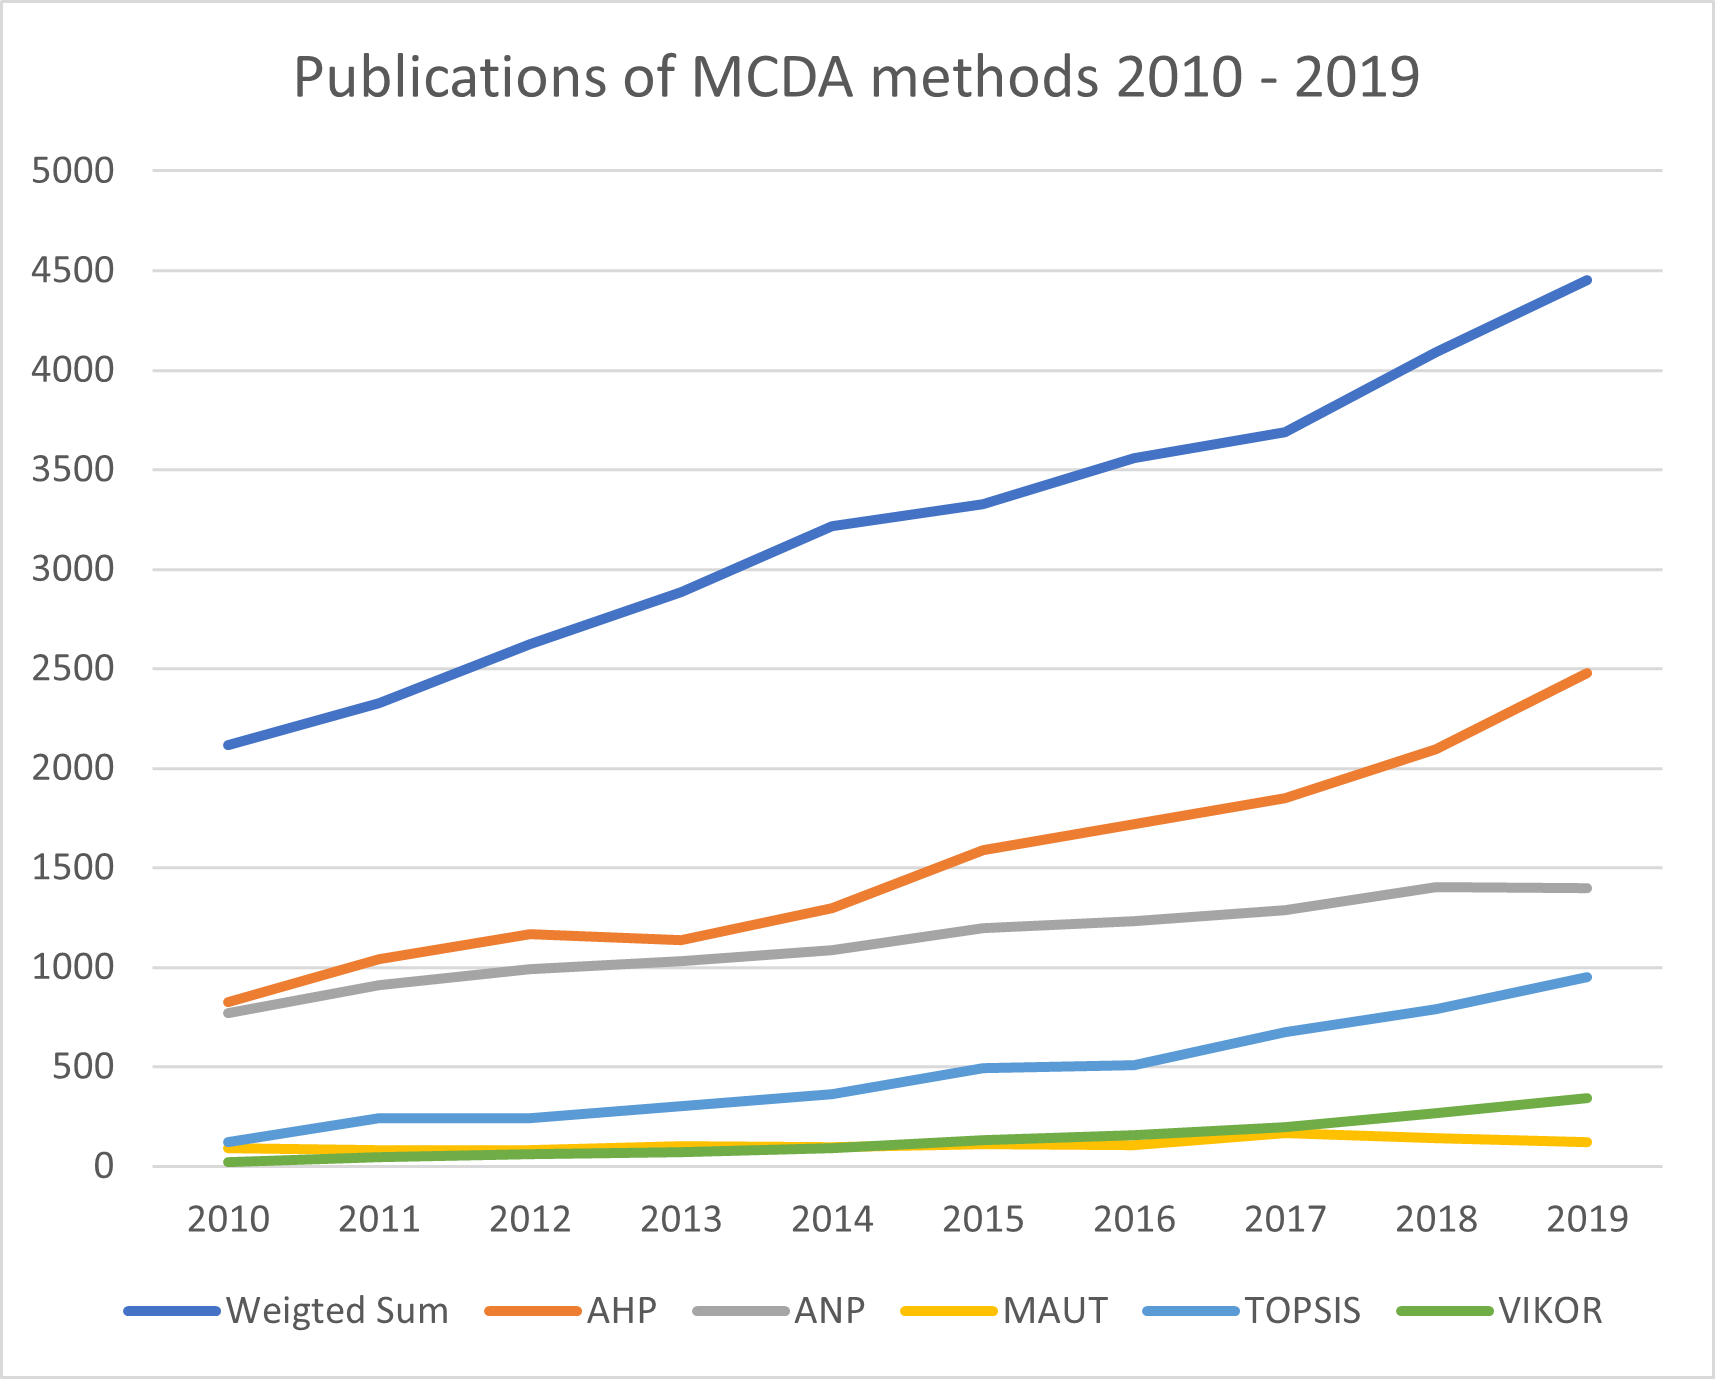
\includegraphics[width=9.5cm]{LUBS5308M Week03 Img001 - MCDA Methods}
	\centering
	\caption{Research outputs showing growing popularity of different MCDA techniques. (Source: Module Learning Material, Week 3)}
    \end{figure}

As the name implies, MCDA allows you to consider multiple conflicting criteria and decide on the best option using different types of information. 
Decisions are incredibly important in industry, especially decisions related to product development.\\
In the following sections, we will understand AHP and TOPSIS one by one with examples.
\section{Analytical Hierarchy Process}
 AHP is a pairwise comparison method, which is an approach to MCDA, in which we compare each alternative/criterion head-to-head with all the other alternatives/criteria and it is up to the decision maker to choose the best comparison.\\
 Saaty also proposed the use of 1-9 scale for AHP when comparing criterion and alternatives in order to facilitate the comparisons and convert qualitative comparisons to a quantitative scale.\\
 It was given by \href{https://en.wikipedia.org/wiki/Thomas_L._Saaty}{Prof. Thomas Saaty} in 1970. \\
\begin{table}[h]
\setlength{\arrayrulewidth}{0.25mm}
\setlength{\tabcolsep}{18pt}
% \renewcommand{\arraystretch}{0.25}
\begin{tabular}{ |p{1cm}|p{3cm}|p{5cm}|  }
\hline
\textbf{Scale}& \textbf{Verbal Expression} &\textbf{Explanation} \\
\hline
1 & Equal Importance & Two criterion are considered to be \textbf{equally} important. \\
\hline
3 & Moderate Importance & One criteria is \textbf{slightly} preferred over the other. \\
\hline
5 & Strong Importance & One criteria is \textbf{strongly} preferred over the other. \\
\hline
7 & Very Very Strong Importance & One criteria is favoured \textbf{very strongly} over another. \\
\hline
9 & Extreme Importance & One criteria is favoured over another with highest affirmation. \\
\hline
\end{tabular}
\caption{\label{tab:table1}1 - 9 Scale used for AHP.}
\end{table} \\
Suppose we are given two critera, $C_j$ and $C_k$. We will first calculate the relative importance of the criteria in decision making. Suppose $a_{j,k}$ is the value captured from the semantic scale(\ref{tab:table1}). The relative importance of $C_k$ over $C_j$ is defined as its reciprocal, i.e, $a_{k,j}$ = 1 / $a_{j,k}$.
A reciprocal matrix {\em A} is then formed using $a_{j,k}$ for all \em j and \em k.
There are two approaches to elicit scores from the reciprocal matrix:
\begin{enumerate}[noitemsep]
    \item Eigenvector method
    \item Geometric mean method
\end{enumerate}
It has been generally agreed that the weights of criteria can be estimated by finding the principal eigenvector $\omega$ of matrix A: 
\begin{center}
{\em \LARGE AW} = \LARGE{$\lambda_{max}\omega$}.
\end{center}
Using similar procedures, the weights of alternatives with respect to each criterion are computed. Then, the overall weights of alternatives are computed using the weighted summation:
\begin{center}

\left( \begin{array}{cc} Overall\:Weight \\
of\:alternative\:i \end{array} \right) =\:\: $\sum_j$
\left( \begin{array}{c} Weight\:of\:alternative\:i\:with \\ respect\:to\: Cj\: X \:Weight\: of\: Cj\: \\ with\: respect\: to\: the\: goal \end{array} \right)

\end{center}

\section{TOPSIS}
TOPSIS, or \textbf{T}echnique for \textbf{O}rder \textbf{P}reference by \textbf{S}imilarity to \textbf{I}deal \textbf{S}olutions,  is an Ideal Point Method, in which we aim to decide the ideal solution by distancing the positive and negative factors. Such methods are intuitive to explain. Before, getting into of TOPSIS, let us first understand what is an Ideal Point Method. \\

Ideal points methods are based on the idea of assessing each alternative that is under consideration based on their separation/distance from either:
\begin{itemize}
    \item \textbf{The most ideal point}: Also known as the \underline{positive ideal point}, represents the \emph{best possible solution} for each criterion and typically corresponds to an imaginary solution that is \textbf{not} feasible in real life. \\
    \textbf{Example}: Getting a business class seat ticket cheaper than a bus ticket.
    \item \textbf{The least ideal point}: Also known as the \underline{negative ideal point}, represents the \emph{worst possible outcome} for each criterion, something that is too bad to happen in real life. \\
    \textbf{Example}: Getting a bus ticket costlier than the most luxurious business class ticket.
\end{itemize}
When applying ideal point methods, another area of consideration is the distance measurement that will be used. 
The following are the most commonly used distance measures: 

\begin{center}

\textbf{Euclidean} = \sqrt {\sum _{i=1}^{n}  \left( q_{i}-p_{i}\right)^2 } \\~\\
\textbf{Manhattan} = (\sum_{i=1}^n |q_i-p_i|)
\\~\\
\textbf{Chebyshev} = \max_{i} (| q_{i} -p_{i}| )

\end{center}

The principle behind TOPSIS is that the optimal alternative should have the \textbf{shortest} distance from the \textbf{Positive Ideal Solution (PIS)} and the \textbf{furhtest} distance from the \textbf{Negative Ideal Solution (NIS)}.
TOPSIS uses the Euclidean distance measure between the actual alternative and the hypothesised one to calculate the result.
\\
To find score of each alternative using TOPSIS, we first formulate a decision matrix with scores depicting the weights(importance) given to each criterion.\\
Then we normalise the decision matrix using vector normalization:
\begin{center}
    
\LARGE{$r_{i,j}$ = $\frac{x_{ij}}{\sqrt{\sum_ix_{ij}^2}}$}\\
\end{center}
where \emph{$x_{ij}$} is the score of alternative \emph{i} with respect to criterion \emph{j}.\\~\\
Using the weighted normal matrix, we can determine the positive ideal solution and the negative ideal solution for each criterion.\\
The best alternative is the one that is closest to PIS and furthest away from NIS. To find that, we calculate the distance between each alternative and PIS / NIS.\\
To start, we can calculate the distance between each alternative to the PIS using the formula: 
\begin{center}
    
\large{$S_i^*$ = $\sqrt{\sum(V_{ij} - V_{j}^*)^2}$} 
\end{center}

In a similar manner, we can also find the distance between each alternative to the NIS using:
\begin{center}
    
\large{$S_i^-$ = $\sqrt{\sum(V_{ij} - V_{j}^-)^2}$} 
\end{center}

Finally, we can calculate the relative closeness to the ideal solution using the following calculation:
\begin{center}
    
\large{\emph{Final Score}} = \LARGE{$\frac{S_i^-}{(S_i^* + S_i^-)}$}
\end{center}
\textbf{The higher the score, the better the alternative, according to TOPSIS!}
\\
\section*{Summary}
Although both AHP and TOPSIS are MCDA techniques, they are based on different methodologies. While AHP is an example of \emph{Pairwise Comparison Method} in which all the alternatives are compared head to head, TOPSIS, on the other hand, is an \emph{Ideal Point Technique} in which the alternative closest to best possible hypothetical scenario and farthest from worst possible hypothetical scenario is selected.\\~\\
Apart from this, both techniques have their own \textbf{limitations}:\\
Both AHP and TOPSIS suffer from \textbf{Rank Reversal Problem}. i.e \textsl{"When the rank of preferability for all alternatives changes when the set of available alternatives changes, either by the introduction of new alternatives or the removal of one."} \\
Apart from this, AHP also has limitations like pairwise consistency and that it can sometimes be too time consuming.\\~\\
Both methods can be used independently for different types of problems. However, many researchers consider that TOPSIS, because its clear and mathematically sound structure is preferred over AHP which mathematical structure has been, and is very criticized. However, AHP is by far the most used method for modern decision making.

\end{document}
